\documentclass[noauthor,nooutcomes,hints,handout]{ximera}

\graphicspath{  
{./}
{./whoAreYou/}
{./drawingWithTheTurtle/}
{./bisectionMethod/}
{./circles/}
{./anglesAndRightTriangles/}
{./lawOfSines/}
{./lawOfCosines/}
{./plotter/}
{./staircases/}
{./pitch/}
{./qualityControl/}
{./symmetry/}
{./nGonBlock/}
}


%% page layout
\usepackage[cm,headings]{fullpage}
\raggedright
\setlength\headheight{13.6pt}


%% fonts
\usepackage{euler}

\usepackage{FiraMono}
\renewcommand\familydefault{\ttdefault} 
\usepackage[defaultmathsizes]{mathastext}
\usepackage[htt]{hyphenat}

\usepackage[T1]{fontenc}
\usepackage[scaled=1]{FiraSans}

%\usepackage{wedn}
\usepackage{pbsi} %% Answer font


\usepackage{cancel} %% strike through in pitch/pitch.tex


%% \usepackage{ulem} %% 
%% \renewcommand{\ULthickness}{2pt}% changes underline thickness

\tikzset{>=stealth}

\usepackage{adjustbox}

\setcounter{titlenumber}{-1}

%% journal style
\makeatletter
\newcommand\journalstyle{%
  \def\activitystyle{activity-chapter}
  \def\maketitle{%
    \addtocounter{titlenumber}{1}%
                {\flushleft\small\sffamily\bfseries\@pretitle\par\vspace{-1.5em}}%
                {\flushleft\LARGE\sffamily\bfseries\thetitlenumber\hspace{1em}\@title \par }%
                {\vskip .6em\noindent\textit\theabstract\setcounter{question}{0}\setcounter{sectiontitlenumber}{0}}%
                    \par\vspace{2em}
                    \phantomsection\addcontentsline{toc}{section}{\thetitlenumber\hspace{1em}\textbf{\@title}}%
                     }}
\makeatother



%% thm like environments
\let\question\relax
\let\endquestion\relax

\newtheoremstyle{QuestionStyle}{\topsep}{\topsep}%%% space between body and thm
		{}                      %%% Thm body font
		{}                              %%% Indent amount (empty = no indent)
		{\bfseries}            %%% Thm head font
		{)}                              %%% Punctuation after thm head
		{ }                           %%% Space after thm head
		{\thmnumber{#2}\thmnote{ \bfseries(#3)}}%%% Thm head spec
\theoremstyle{QuestionStyle}
\newtheorem{question}{}



\let\freeResponse\relax
\let\endfreeResponse\relax

%% \newtheoremstyle{ResponseStyle}{\topsep}{\topsep}%%% space between body and thm
%% 		{\wedn\bfseries}                      %%% Thm body font
%% 		{}                              %%% Indent amount (empty = no indent)
%% 		{\wedn\bfseries}            %%% Thm head font
%% 		{}                              %%% Punctuation after thm head
%% 		{3ex}                           %%% Space after thm head
%% 		{\underline{\underline{\thmname{#1}}}}%%% Thm head spec
%% \theoremstyle{ResponseStyle}

\usepackage[tikz]{mdframed}
\mdfdefinestyle{ResponseStyle}{leftmargin=1cm,linecolor=black,roundcorner=5pt,
, font=\bsifamily,}%font=\wedn\bfseries\upshape,}


\ifhandout
\NewEnviron{freeResponse}{}
\else
%\newtheorem{freeResponse}{Response:}
\newenvironment{freeResponse}{\begin{mdframed}[style=ResponseStyle]}{\end{mdframed}}
\fi



%% attempting to automate outcomes.

%% \newwrite\outcomefile
%%   \immediate\openout\outcomefile=\jobname.oc
%% \renewcommand{\outcome}[1]{\edef\theoutcomes{\theoutcomes #1~}%
%% \immediate\write\outcomefile{\unexpanded{\outcome}{#1}}}

%% \newcommand{\outcomelist}{\begin{itemize}\theoutcomes\end{itemize}}

%% \NewEnviron{listOutcomes}{\small\sffamily
%% After answering the following questions, students should be able to:
%% \begin{itemize}
%% \BODY
%% \end{itemize}
%% }
\usepackage[tikz]{mdframed}
\mdfdefinestyle{OutcomeStyle}{leftmargin=2cm,rightmargin=2cm,linecolor=black,roundcorner=5pt,
, font=\small\sffamily,}%font=\wedn\bfseries\upshape,}
\newenvironment{listOutcomes}{\begin{mdframed}[style=OutcomeStyle]After answering the following questions, students should be able to:\begin{itemize}}{\end{itemize}\end{mdframed}}



%% my commands

\newcommand{\snap}{{\bfseries\itshape\textsf{Snap!}}}
\newcommand{\flavor}{\link[\snap]{https://snap.berkeley.edu/}}
\newcommand{\mooculus}{\textsf{\textbf{MOOC}\textnormal{\textsf{ULUS}}}}


\usepackage{tkz-euclide}
\tikzstyle geometryDiagrams=[rounded corners=.5pt,ultra thick,color=black]
\colorlet{penColor}{black} % Color of a curve in a plot



\ifhandout\newcommand{\mynewpage}{\newpage}\else\newcommand{\mynewpage}{}\fi


\title{Stars}
\author{Jenny Sheldon \and Bart Snapp}

\begin{document}
\begin{abstract}
  We explore the mathematics of drawing stars.
\end{abstract}
\maketitle

\begin{listOutcomes}
\item Draw simple $n$-sided pictures of maximal dihedral symmetry.
\item Draw stars with $n$-sides.
\item Analyze the properties of $n$-sided stars.
\item Demonstrate a working understanding with stars and star notation.
\end{listOutcomes}

Can you remember when you first learned to draw a star? I can! I was first taught to draw a star like this:
\[
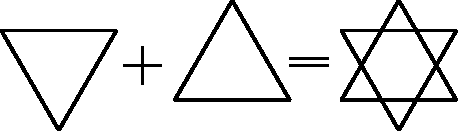
\includegraphics{bartTri.pdf}
\]
But I wanted to know how to draw 5-pointed stars like the other
kids. So one day I taught myself to draw a star like this:
\[
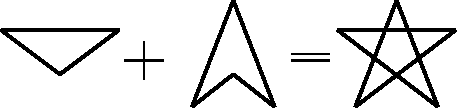
\includegraphics{bartTri2.pdf}
\]
This may seem like a silly way to draw this star---it certainly makes
me chuckle now. Let's see if we can give a theory for drawing stars
that will connect the two different stars above, teach you how to
draw some new stars, and learn a little more mathematics along the
way.


We'll start with $5$ points equally spaced on a circle:
\[
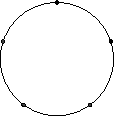
\includegraphics{stfive.pdf}
\]
Think of these points as \textit{pins}.  Next we'll start at the top
and draw lines that we'll think of as \textit{strings}, moving
clockwise to the point two steps away each time:
\[
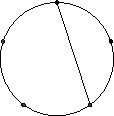
\includegraphics{stfive1.pdf}\qquad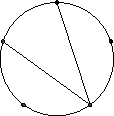
\includegraphics{stfive2.pdf}\qquad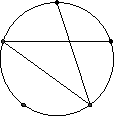
\includegraphics{stfive3.pdf}\qquad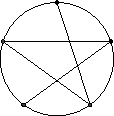
\includegraphics{stfive4.pdf}\qquad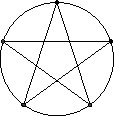
\includegraphics{stfive5.pdf}
\]
Check it out, we got a star! If we had used pins and string to make
this star, we could have done it with one piece of string.



Now start with $6$ points equally spaced on a circle. Again, we'll
move clockwise two steps each time:
\[
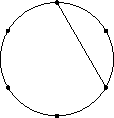
\includegraphics{stsix1.pdf}\qquad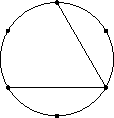
\includegraphics{stsix2.pdf}\qquad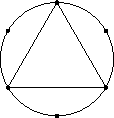
\includegraphics{stsix3.pdf}
\]
Oops, we've run out of points! No worries, just start again at one of
the points that hasn't been touched by a line yet, drawing lines and
moving two steps each time:
\[
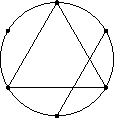
\includegraphics{stsix4.pdf}\qquad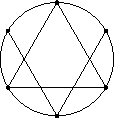
\includegraphics{stsix5.pdf}\qquad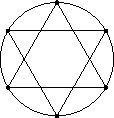
\includegraphics{stsix6.pdf}
\]
Ah! The other star! In this case, if we used pins and strings, we'd
need to use \textit{two} pieces of string.


I'm hoping that the following notation will help out:
\[
\stringstar{n}{s}=\left[\begin{minipage}{3.7in}
the star with $n$ equally spaced points where we move $s$ steps clockwise
\end{minipage}\right]
\]
Remember, $\stringstar{n}{s}$ is a star, \textbf{not} a fraction!
Stars can be drawn in \snap\ with this block:
\begin{center}
  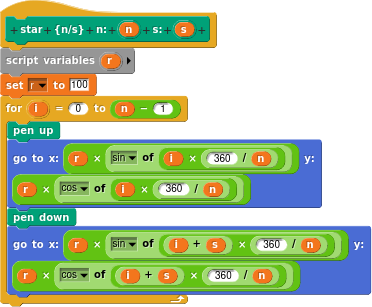
\includegraphics[width=3in]{starBlockScript.png}
\end{center}





\mynewpage






\begin{question}
  Some stars with different numbers look the same. For example:
  \[
  \stringstar{12}{3}\quad\text{and}\quad\stringstar{12}{9}
  \]
look the same.  Use
\raisebox{-.4\height}{
\includegraphics{starBlock.png}} to investigate
which stars look the same.
\begin{enumerate}
  \item Assume that $0 < s < t< n$.  GIVE A GENERAL RULE for when the
    stars stars $\stringstar{n}{s}$ and $\stringstar{n}{t}$ look the
    same.
  \item EXPLAIN WHY your rule is true.
  \item What if $s$ or $t$ are bigger than $n$? MODIFY your rule to
    account for this and EXPLAIN WHY your new rule is true.
\end{enumerate}
\begin{freeResponse}
  \begin{enumerate}
  \item A star $\stringstar{n}{s}$ looks the same as $\stringstar{n}{t}$ for
    $0 < s < t< n$ when $n=s+ t$.
  \item This is true, because you are just drawing the star ``backwards.''
  \item If $s$ and $t$ can be bigger than $n$, then we modify the
    rule to be: A star $\stringstar{n}{s}$ looks the same as
    $\stringstar{n}{t}$ for $0 < s < t< n$ when $n$ is a factor of
    $s+t$. In essence, we just spin around the circle more times
    before we put our point down.
  \end{enumerate}
\end{freeResponse}
\end{question}
\mynewpage

\begin{question}
  \begin{enumerate}
  \item Give a precise DESCRIPTION of what happens when we ``reduce to
    lowest terms.'' As an example, think about how the stars
    $\stringstar{6}{2}$ and $\stringstar{3}{1}$ are related.
  \item EXPLAIN WHY your description holds.
  \end{enumerate}
  As a gesture of friendship, I suggest you check out (and play with!)
  this script:
  \begin{center}
    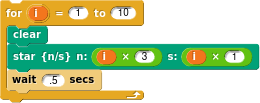
\includegraphics{starSeq.png}
  \end{center}
  \begin{freeResponse}
    \begin{enumerate}
      \item When we ``reduce'' a star, we find the piece it is made
        of.  The star
        \[
        \stringstar{12}{4}
        \]
        is made of pieces of $\stringstar{3}{1}$, and the fraction
        \[
        \frac{12}{4} = \frac{3}{1}.
        \]
      \item This happens, because of how stars work, and how fractions reduce.
        \[
        \frac{x\cdot p}{y\cdot p} =  \frac{x}{y}.
        \]
        This is how fractions reduce. On the other hand, with stars,
        if $n=x\cdot p$, and $s=y\cdot p$, then we must have a
        $\stringstar{x}{y}$ star as part of the star
        $\stringstar{x\cdot p}{y\cdot q}$, as we are traveling from a
        point on the circle to a point that is
        \[
        \frac{x\cdot p}{y\cdot q} =  \frac{x}{y}
        \]
        further clockwise on the circle.
    \end{enumerate}
  \end{freeResponse}
\end{question}

\mynewpage


\begin{question}
%%  For a fixed value of $n$ how many stars could be drawn with a single
%%  piece of string? euler phi...
  Demonstrate a working understanding by using the following script
  \begin{center}
    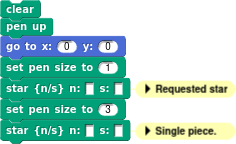
\includegraphics{starsSubBLANKScript.png}
  \end{center}
  to draw the following stars for me:
  \begin{enumerate}
  \item A star, made of $3$ separate $\stringstar{5}{2}$ stars.
   \item A star, with $21$ points and $7$ pieces. 
   \item A star, with $21$ points made of separate $\stringstar{7}{2}$
     stars.
  \end{enumerate}
  Use \snap\ to show off your work by giving screenshots of your
  SCRIPTS and STAGES.
  \begin{freeResponse}
    Here they are:
    \begin{enumerate}
    \item
      \begin{center}
        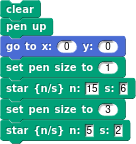
\includegraphics[width=.3\textwidth]{starsSub15-5-2Script.png}   \qquad \fbox{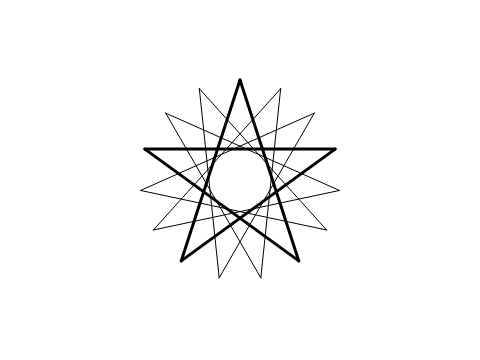
\includegraphics[width=.3\textwidth]{starsSub15-5-2Stage.png}}
      \end{center}
    \item
      \begin{center}
        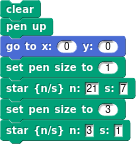
\includegraphics[width=.3\textwidth]{starsSub21-3-1Script.png}   \qquad \fbox{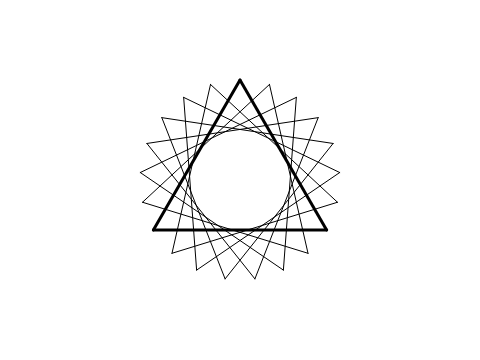
\includegraphics[width=.3\textwidth]{starsSub21-3-1Stage.png}}
      \end{center}
    \item \begin{center}
      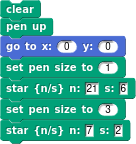
\includegraphics[width=.3\textwidth]{starsSub21-7-2Script.png}   \qquad \fbox{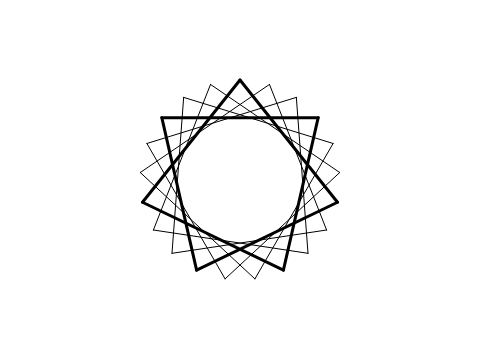
\includegraphics[width=.3\textwidth]{starsSub21-7-2Stage.png}}
    \end{center}
    \end{enumerate}
  \end{freeResponse}
\end{question}
\end{document}
